\documentclass{beamer}

\usepackage{biblatex}

\usetheme{Copenhagen}
%Information to be included in the title page:
\title[Road Fatalities and Safety Features]{The Effect of Advanced Safety Features on Crash Fatality Rates for Vulnerable Road Users}
\addbibresource{traffic.bib}
\author{Matt McAnear}
\institute{University of Michigan}
\date{\today}

\begin{document}

\frame{\titlepage}

\begin{frame}
\frametitle{Introduction}

\begin{itemize}
    \item Cars are getting bigger\cite{kovach_rise_2021}
    \item Cars are getting more safety features. 
    \item Pedestrian deaths are increasing\cite{tyndall_effect_2024}
    \item What's the effect of advanced safety features for people \textit{outside} the car in the age of increasing car size?
\end{itemize}
\end{frame}

\section{Data}

\begin{frame}{Source}
National Highway Transportation Safety Administration (NHTSA) 
\begin{itemize}
    \item Crash Reporting Statistical System (CRSS)
    \begin{itemize}
        \item 60 subregions in the US
        \item Survey weights reported to aggregate to national level statistics
    \end{itemize}
    \item Fatal Accident Reporting System (FARS) 
    \begin{itemize}
        \item Complete accounting of fatal accidents across the country
    \end{itemize}
\end{itemize}

\end{frame}

\begin{frame}{Simplifications}
\begin{itemize}
    \item Collapse vehicle types into broader categories
    \item Recode states from FARS into regions that align with CRSS
    \item Consider only crashes with a single vehicle and either a pedestrian or cyclist.
    \item Do not consider motorcycle accidents.
    \item Total Effect: Possible systematic reduction in overall fatality rates by removing more fatal accidents.
\end{itemize}
\end{frame}

\begin{frame}{Features of Interest}
    \begin{itemize}
        \item Bodyclass
            \begin{itemize}
                \item \textbf{Vans}= Van, Cargo Van
                \item \textbf{Truck} = Incomplete - Chassis Cab (Single Cab), Truck-Tractor, Truck, Bus
                \item \textbf{Cars} = Hatchback/Liftback/Notchback, Sedan/Saloon, Coupe, Convertible/Cabriolet
            \end{itemize}
        \item Control (Environmental)
            \begin{itemize}
                \item Weather Name (inclement yes/no, unknown)
                \item Light Conditions (Dusk/Daylight, Dark/Night)
            \end{itemize}
        \item Safety - many features, high sparsity
            \begin{itemize}
                \item Pedestrian Auto Emergency Braking
                \item Lane Keeping Assistance
                \item Lane Departure Warning
                \item Backup Camera
                \item Auto Pedestrian Alerting Sound
                \item Anti-Lock Braking System
            \end{itemize}
    \end{itemize}
\end{frame}


\section{Methodology}

\begin{frame}{Logistic Regression}

\begin{equation}
\sigma(Y) = \beta_0[X_j, X_r] + \Big((\pi \odot \beta_{j})[X_j, \dots]\Big) \odot X
\end{equation}

\begin{itemize}
    \item $\sigma(Y)$ is the Logistic transformation, $X_j$ is an indicator for cyclists and $X_r$ is an indicator for region.
    \item $\beta_0$ is a $2 \times 4$ hierarchical matrix of intercepts for region and pedestrians/cyclists.
    \item $\beta_j$ is a $2 \times K$ hierarchical matrix of coefficients for effects between cyclists and pedestrians.  
    \item $\pi$ is a binary vector we use to turn on/off multiple features. It is the 
    same across pedestrians and cyclists.
    \item We create an $N \times K$ matrix of beta coefficients
    and take the dot product with our features $X$ to estimate the logits 
\end{itemize}

\end{frame}

\begin{frame}{Packages}

\begin{itemize}

\item Utilizes hierarchical structure and discrete random variables
for inclusion and exclusion of features for model averaging. 
\item Utilize Numpyro\cite{phan_composable_2019} for the NUTS + DiscreteHMCGibbs sampler classes that allows us to implement the model averaging alongside hierarchical components.
\item Track deterministic components, including $R^2$, from run to run.

\end{itemize}

Used BMA\cite{raftery_bma_2022} as a quick check (not included in paper), and 
found that our methodology improved $R^2$ results marginally.
\end{frame}


\begin{frame}{Diagnostics}
    \centering
    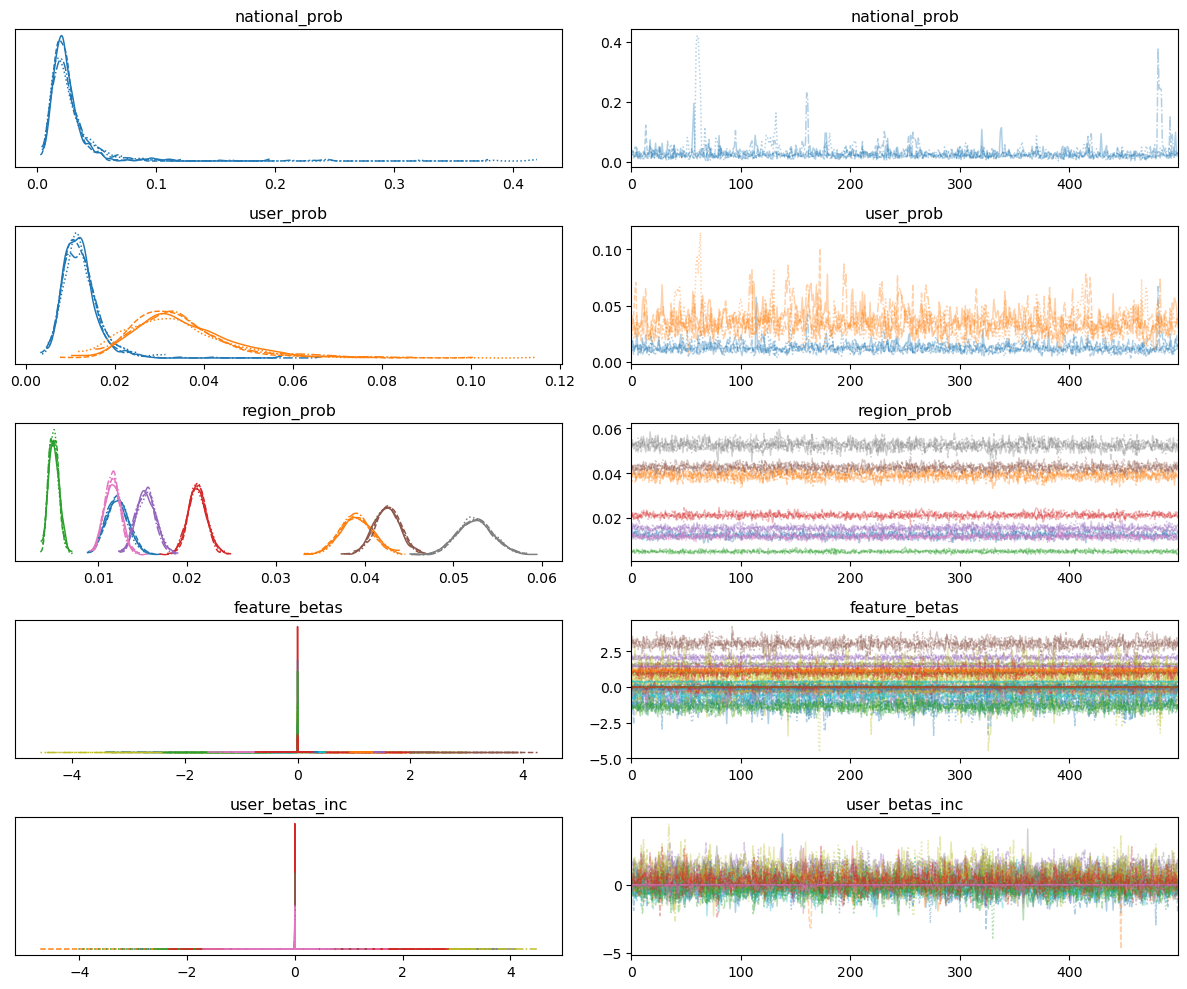
\includegraphics[width=0.7\linewidth]{paper/images/traceplot.png}
\end{frame}


\section{Results}
\begin{frame}{Results}

\textbf{Summary}

Safety features can make a difference, but any effects are:

\begin{enumerate}
    \item Marginal in comparison to the control factors
    \item Indicate model misspecification that cannot be easily resolved.
\end{enumerate}

\end{frame}


\subsection{Coefficients}
\begin{frame}
    \centering
    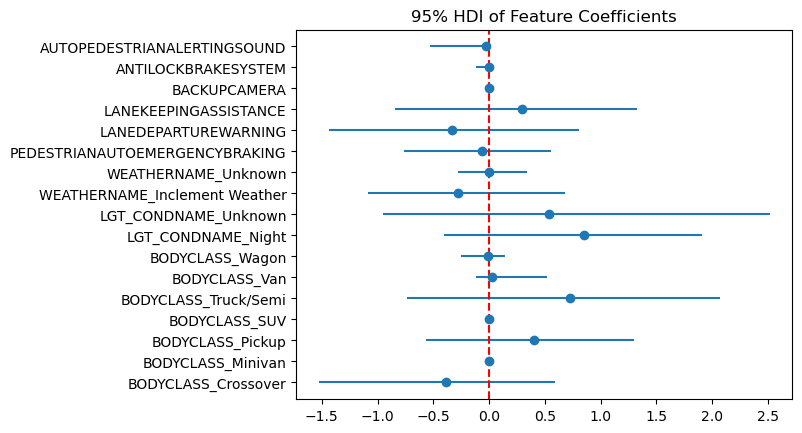
\includegraphics[width=\linewidth]{paper/images/all_users_coefficients.png}
\end{frame}

\begin{frame}
    \centering
    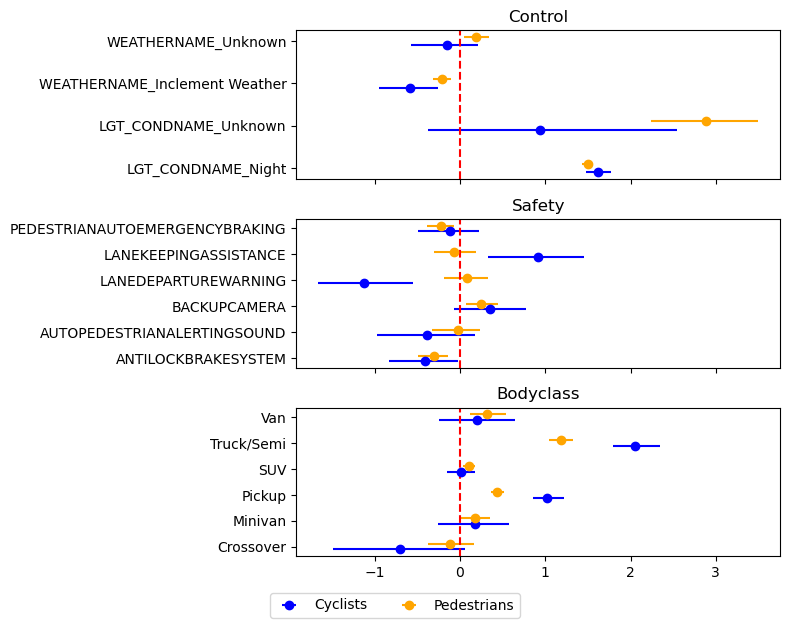
\includegraphics[width=0.9\linewidth]{paper/images/feature_coefficients.png}
\end{frame}

\begin{frame}
\begin{figure}
    \centering
    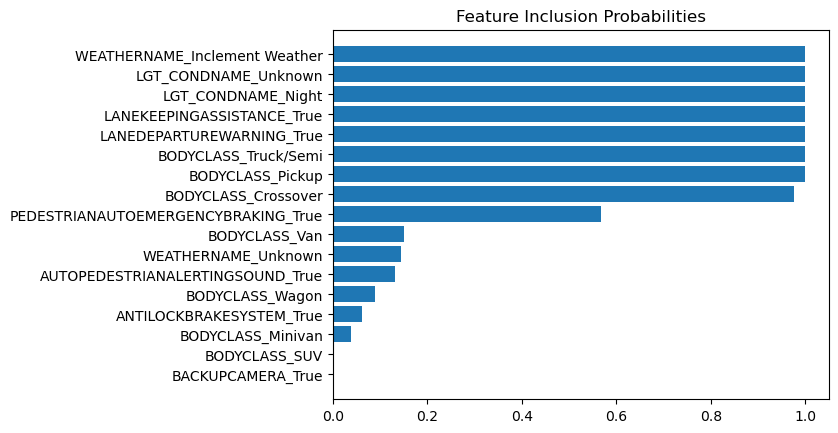
\includegraphics[width=\linewidth]{paper/images/inclusion_probs.png}
\end{figure}
\end{frame}

\begin{frame}
    \begin{figure}
     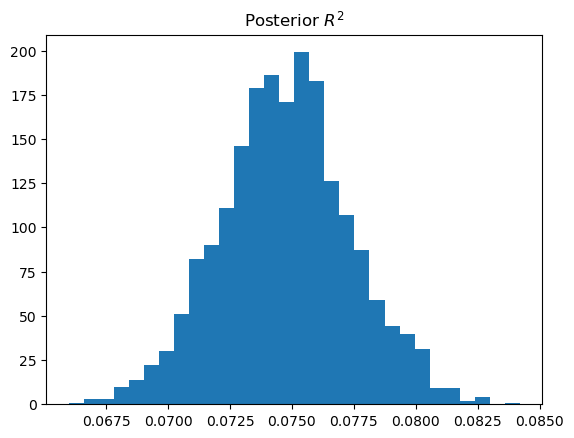
\includegraphics[width=0.7\linewidth]{paper/images/R2_dist.png}
    \centering
    \caption{$R^2$ statistic calculated based on variance in logits alongside variance estimated variance from posterior probabilities. See Gelman et. al\cite{gelman_r-squared_2019}}.
    \label{fig:r2-dist}
    \end{figure}
\end{frame}


\section{Conclusion}

\begin{frame}{Major Findings}

\begin{enumerate}
    \item Our model explains a small proportion of the variance.
    \item Some features have predictable and sensible values, others are counter-intuitive or unlikely.
    \item Region, vehicle size, and environmental factors explain more of the fatality
    risk than almost all safety features (but we don't really trust the remaining one)
    \item Analysis is potentially affected by survey weights and our chosen subsetting.
\end{enumerate}

\end{frame}

\begin{frame}[allowframebreaks]{References}


\printbibliography
    
\end{frame}

\end{document}